%% bare_conf.tex
%% V1.4b
%% 2015/08/26
%% by Michael Shell
%% See:
%% http://www.michaelshell.org/
%% for current contact information.
%%
%% This is a skeleton file demonstrating the use of IEEEtran.cls
%% (requires IEEEtran.cls version 1.8b or later) with an IEEE
%% conference paper.
%%
%% Support sites:
%% http://www.michaelshell.org/tex/ieeetran/
%% http://www.ctan.org/pkg/ieeetran
%% and
%% http://www.ieee.org/

%%*************************************************************************
%% Legal Notice:
%% This code is offered as-is without any warranty either expressed or
%% implied; without even the implied warranty of MERCHANTABILITY or
%% FITNESS FOR A PARTICULAR PURPOSE! 
%% User assumes all risk.
%% In no event shall the IEEE or any contributor to this code be liable for
%% any damages or losses, including, but not limited to, incidental,
%% consequential, or any other damages, resulting from the use or misuse
%% of any information contained here.
%%
%% All comments are the opinions of their respective authors and are not
%% necessarily endorsed by the IEEE.
%%
%% This work is distributed under the LaTeX Project Public License (LPPL)
%% ( http://www.latex-project.org/ ) version 1.3, and may be freely used,
%% distributed and modified. A copy of the LPPL, version 1.3, is included
%% in the base LaTeX documentation of all distributions of LaTeX released
%% 2003/12/01 or later.
%% Retain all contribution notices and credits.
%% ** Modified files should be clearly indicated as such, including  **
%% ** renaming them and changing author support contact information. **
%%*************************************************************************


% *** Authors should verify (and, if needed, correct) their LaTeX system  ***
% *** with the testflow diagnostic prior to trusting their LaTeX platform ***
% *** with production work. The IEEE's font choices and paper sizes can   ***
% *** trigger bugs that do not appear when using other class files.       ***                          ***
% The testflow support page is at:
% http://www.michaelshell.org/tex/testflow/



\documentclass[conference]{IEEEtran}
\usepackage{graphicx}  
\usepackage[margin=2.5cm]{geometry}
\usepackage{breakcites}
\usepackage{indentfirst}
\usepackage{pgfgantt}
\usepackage{pdflscape}
\usepackage{float}
\usepackage{epsfig}
\usepackage{epstopdf}
\usepackage{hyperref}
\usepackage[cmex10]{amsmath}
\usepackage{stfloats}
\usepackage{multirow}
\usepackage{appendix}
\usepackage{listings}
\usepackage{xcolor}
\usepackage{longtable}
\usepackage{booktabs} % For formal tables
% Some Computer Society conferences also require the compsoc mode option,
% but others use the standard conference format.
%
% If IEEEtran.cls has not been installed into the LaTeX system files,
% manually specify the path to it like:
% \documentclass[conference]{../sty/IEEEtran}





% Some very useful LaTeX packages include:
% (uncomment the ones you want to load)


% *** MISC UTILITY PACKAGES ***
%
%\usepackage{ifpdf}
% Heiko Oberdiek's ifpdf.sty is very useful if you need conditional
% compilation based on whether the output is pdf or dvi.
% usage:
% \ifpdf
%   % pdf code
% \else
%   % dvi code
% \fi
% The latest version of ifpdf.sty can be obtained from:
% http://www.ctan.org/pkg/ifpdf
% Also, note that IEEEtran.cls V1.7 and later provides a builtin
% \ifCLASSINFOpdf conditional that works the same way.
% When switching from latex to pdflatex and vice-versa, the compiler may
% have to be run twice to clear warning/error messages.






% *** CITATION PACKAGES ***
%
%\usepackage{cite}
% cite.sty was written by Donald Arseneau
% V1.6 and later of IEEEtran pre-defines the format of the cite.sty package
% \cite{} output to follow that of the IEEE. Loading the cite package will
% result in citation numbers being automatically sorted and properly
% "compressed/ranged". e.g., [1], [9], [2], [7], [5], [6] without using
% cite.sty will become [1], [2], [5]--[7], [9] using cite.sty. cite.sty's
% \cite will automatically add leading space, if needed. Use cite.sty's
% noadjust option (cite.sty V3.8 and later) if you want to turn this off
% such as if a citation ever needs to be enclosed in parenthesis.
% cite.sty is already installed on most LaTeX systems. Be sure and use
% version 5.0 (2009-03-20) and later if using hyperref.sty.
% The latest version can be obtained at:
% http://www.ctan.org/pkg/cite
% The documentation is contained in the cite.sty file itself.






% *** GRAPHICS RELATED PACKAGES ***
%
\ifCLASSINFOpdf
  % \usepackage[pdftex]{graphicx}
  % declare the path(s) where your graphic files are
  % \graphicspath{{../pdf/}{../jpeg/}}
  % and their extensions so you won't have to specify these with
  % every instance of \includegraphics
  % \DeclareGraphicsExtensions{.pdf,.jpeg,.png}
\else
  % or other class option (dvipsone, dvipdf, if not using dvips). graphicx
  % will default to the driver specified in the system graphics.cfg if no
  % driver is specified.
  % \usepackage[dvips]{graphicx}
  % declare the path(s) where your graphic files are
  % \graphicspath{{../eps/}}
  % and their extensions so you won't have to specify these with
  % every instance of \includegraphics
  % \DeclareGraphicsExtensions{.eps}
\fi
% graphicx was written by David Carlisle and Sebastian Rahtz. It is
% required if you want graphics, photos, etc. graphicx.sty is already
% installed on most LaTeX systems. The latest version and documentation
% can be obtained at: 
% http://www.ctan.org/pkg/graphicx
% Another good source of documentation is "Using Imported Graphics in
% LaTeX2e" by Keith Reckdahl which can be found at:
% http://www.ctan.org/pkg/epslatex
%
% latex, and pdflatex in dvi mode, support graphics in encapsulated
% postscript (.eps) format. pdflatex in pdf mode supports graphics
% in .pdf, .jpeg, .png and .mps (metapost) formats. Users should ensure
% that all non-photo figures use a vector format (.eps, .pdf, .mps) and
% not a bitmapped formats (.jpeg, .png). The IEEE frowns on bitmapped formats
% which can result in "jaggedy"/blurry rendering of lines and letters as
% well as large increases in file sizes.
%
% You can find documentation about the pdfTeX application at:
% http://www.tug.org/applications/pdftex





% *** MATH PACKAGES ***
%
%\usepackage{amsmath}
% A popular package from the American Mathematical Society that provides
% many useful and powerful commands for dealing with mathematics.
%
% Note that the amsmath package sets \interdisplaylinepenalty to 10000
% thus preventing page breaks from occurring within multiline equations. Use:
%\interdisplaylinepenalty=2500
% after loading amsmath to restore such page breaks as IEEEtran.cls normally
% does. amsmath.sty is already installed on most LaTeX systems. The latest
% version and documentation can be obtained at:
% http://www.ctan.org/pkg/amsmath





% *** SPECIALIZED LIST PACKAGES ***
%
%\usepackage{algorithmic}
% algorithmic.sty was written by Peter Williams and Rogerio Brito.
% This package provides an algorithmic environment fo describing algorithms.
% You can use the algorithmic environment in-text or within a figure
% environment to provide for a floating algorithm. Do NOT use the algorithm
% floating environment provided by algorithm.sty (by the same authors) or
% algorithm2e.sty (by Christophe Fiorio) as the IEEE does not use dedicated
% algorithm float types and packages that provide these will not provide
% correct IEEE style captions. The latest version and documentation of
% algorithmic.sty can be obtained at:
% http://www.ctan.org/pkg/algorithms
% Also of interest may be the (relatively newer and more customizable)
% algorithmicx.sty package by Szasz Janos:
% http://www.ctan.org/pkg/algorithmicx




% *** ALIGNMENT PACKAGES ***
%
%\usepackage{array}
% Frank Mittelbach's and David Carlisle's array.sty patches and improves
% the standard LaTeX2e array and tabular environments to provide better
% appearance and additional user controls. As the default LaTeX2e table
% generation code is lacking to the point of almost being broken with
% respect to the quality of the end results, all users are strongly
% advised to use an enhanced (at the very least that provided by array.sty)
% set of table tools. array.sty is already installed on most systems. The
% latest version and documentation can be obtained at:
% http://www.ctan.org/pkg/array


% IEEEtran contains the IEEEeqnarray family of commands that can be used to
% generate multiline equations as well as matrices, tables, etc., of high
% quality.




% *** SUBFIGURE PACKAGES ***
%\ifCLASSOPTIONcompsoc
%  \usepackage[caption=false,font=normalsize,labelfont=sf,textfont=sf]{subfig}
%\else
%  \usepackage[caption=false,font=footnotesize]{subfig}
%\fi
% subfig.sty, written by Steven Douglas Cochran, is the modern replacement
% for subfigure.sty, the latter of which is no longer maintained and is
% incompatible with some LaTeX packages including fixltx2e. However,
% subfig.sty requires and automatically loads Axel Sommerfeldt's caption.sty
% which will override IEEEtran.cls' handling of captions and this will result
% in non-IEEE style figure/table captions. To prevent this problem, be sure
% and invoke subfig.sty's "caption=false" package option (available since
% subfig.sty version 1.3, 2005/06/28) as this is will preserve IEEEtran.cls
% handling of captions.
% Note that the Computer Society format requires a larger sans serif font
% than the serif footnote size font used in traditional IEEE formatting
% and thus the need to invoke different subfig.sty package options depending
% on whether compsoc mode has been enabled.
%
% The latest version and documentation of subfig.sty can be obtained at:
% http://www.ctan.org/pkg/subfig




% *** FLOAT PACKAGES ***
%
%\usepackage{fixltx2e}
% fixltx2e, the successor to the earlier fix2col.sty, was written by
% Frank Mittelbach and David Carlisle. This package corrects a few problems
% in the LaTeX2e kernel, the most notable of which is that in current
% LaTeX2e releases, the ordering of single and double column floats is not
% guaranteed to be preserved. Thus, an unpatched LaTeX2e can allow a
% single column figure to be placed prior to an earlier double column
% figure.
% Be aware that LaTeX2e kernels dated 2015 and later have fixltx2e.sty's
% corrections already built into the system in which case a warning will
% be issued if an attempt is made to load fixltx2e.sty as it is no longer
% needed.
% The latest version and documentation can be found at:
% http://www.ctan.org/pkg/fixltx2e


%\usepackage{stfloats}
% stfloats.sty was written by Sigitas Tolusis. This package gives LaTeX2e
% the ability to do double column floats at the bottom of the page as well
% as the top. (e.g., "\begin{figure*}[!b]" is not normally possible in
% LaTeX2e). It also provides a command:
%\fnbelowfloat
% to enable the placement of footnotes below bottom floats (the standard
% LaTeX2e kernel puts them above bottom floats). This is an invasive package
% which rewrites many portions of the LaTeX2e float routines. It may not work
% with other packages that modify the LaTeX2e float routines. The latest
% version and documentation can be obtained at:
% http://www.ctan.org/pkg/stfloats
% Do not use the stfloats baselinefloat ability as the IEEE does not allow
% \baselineskip to stretch. Authors submitting work to the IEEE should note
% that the IEEE rarely uses double column equations and that authors should try
% to avoid such use. Do not be tempted to use the cuted.sty or midfloat.sty
% packages (also by Sigitas Tolusis) as the IEEE does not format its papers in
% such ways.
% Do not attempt to use stfloats with fixltx2e as they are incompatible.
% Instead, use Morten Hogholm'a dblfloatfix which combines the features
% of both fixltx2e and stfloats:
%
% \usepackage{dblfloatfix}
% The latest version can be found at:
% http://www.ctan.org/pkg/dblfloatfix




% *** PDF, URL AND HYPERLINK PACKAGES ***
%
%\usepackage{url}
% url.sty was written by Donald Arseneau. It provides better support for
% handling and breaking URLs. url.sty is already installed on most LaTeX
% systems. The latest version and documentation can be obtained at:
% http://www.ctan.org/pkg/url
% Basically, \url{my_url_here}.




% *** Do not adjust lengths that control margins, column widths, etc. ***
% *** Do not use packages that alter fonts (such as pslatex).         ***
% There should be no need to do such things with IEEEtran.cls V1.6 and later.
% (Unless specifically asked to do so by the journal or conference you plan
% to submit to, of course. )


% correct bad hyphenation here
\hyphenation{op-tical net-works semi-conduc-tor}


\begin{document}
%
% paper title
% Titles are generally capitalized except for words such as a, an, and, as,
% at, but, by, for, in, nor, of, on, or, the, to and up, which are usually
% not capitalized unless they are the first or last word of the title.
% Linebreaks \\ can be used within to get better formatting as desired.
% Do not put math or special symbols in the title.
\title{
    Memalloc as an Alternative for Malloc
}


% author names and affiliations
% use a multiple column layout for up to three different
% affiliations
\author{\IEEEauthorblockN{Fırat Kızılboğa}
\IEEEauthorblockA{Computer Engineering\\
Istanbul Technical University\\
Istanbul, Turkey\\
kizilboga20@itu.edu.tr}}



% conference papers do not typically use \thanks and this command
% is locked out in conference mode. If really needed, such as for
% the acknowledgment of grants, issue a \IEEEoverridecommandlockouts
% after \documentclass

% for over three affiliations, or if they all won't fit within the width
% of the page, use this alternative format:
% 
%\author{\IEEEauthorblockN{Michael Shell\IEEEauthorrefmark{1},
%Homer Simpson\IEEEauthorrefmark{2},
%James Kirk\IEEEauthorrefmark{3}, 
%Montgomery Scott\IEEEauthorrefmark{3} and
%Eldon Tyrell\IEEEauthorrefmark{4}}
%\IEEEauthorblockA{\IEEEauthorrefmark{1}School of Electrical and Computer Engineering\\
%Georgia Institute of Technology,
%Atlanta, Georgia 30332--0250\\ Email: see http://www.michaelshell.org/contact.html}
%\IEEEauthorblockA{\IEEEauthorrefmark{2}Twentieth Century Fox, Springfield, USA\\
%Email: homer@thesimpsons.com}
%\IEEEauthorblockA{\IEEEauthorrefmark{3}Starfleet Academy, San Francisco, California 96678-2391\\
%Telephone: (800) 555--1212, Fax: (888) 555--1212}
%\IEEEauthorblockA{\IEEEauthorrefmark{4}Tyrell Inc., 123 Replicant Street, Los Angeles, California 90210--4321}}




% use for special paper notices
%\IEEEspecialpapernotice{(Invited Paper)}




% make the title area
\maketitle

% As a general rule, do not put math, special symbols or citations
% in the abstract
\begin{abstract}
In contemporary computer systems, efficient memory management is pivotal for performance optimization. This paper introduces a bespoke memory management system that supplants the standard malloc and free operations with customized functions designed to better utilize system memory through various allocation strategies. The system initializes with a heap of a user-defined size, aligned to the system's page size using mmap. We then detail the implementation of MyMalloc, which supports four distinct memory allocation strategies: Bestfit, Worstfit, Firstfit, and Nextfit, enabling dynamic memory management according to user-selected criteria. Correspondingly, MyFree is used to deallocate memory and coalesce free memory spaces, thus optimizing subsequent allocations. The DumpFreeList function is utilized for debugging, providing a clear visualization of the heap's state at any moment. The system's robustness is demonstrated through controlled experiments where memory processes are dynamically allocated and deallocated, showcasing the effectiveness of each strategy and the overall system in managing memory efficiently. The results highlight the nuances between mmap and traditional malloc, with the former offering more precise control over memory allocation, essential for high-performance applications.
\end{abstract}
% no keywords




% For peer review papers, you can put extra information on the cover
% page as needed:
% \ifCLASSOPTIONpeerreview
% \begin{center} \bfseries EDICS Category: 3-BBND \end{center}
% \fi
%
% For peerreview papers, this IEEEtran command inserts a page break and
% creates the second title. It will be ignored for other modes.
\IEEEpeerreviewmaketitle



\section{Introduction}
Efficient memory management is a cornerstone of high-performance computing systems, directly impacting application responsiveness and system stability. Traditional memory management techniques, while robust, often fall short in harnessing the full potential of modern hardware capabilities. This shortfall motivates the development of more adaptable and hardware-conscious strategies that can dynamically manage memory in ways that are both efficient and suited to specific application needs.

In this paper, we present a custom memory management system designed to replace the conventional malloc and free functions with MyMalloc and MyFree. These functions are tailored to offer flexible memory allocation and deallocation strategies that adapt to varied application demands and system states. The initialization of this system relies on mmap, a memory mapping technique that grants direct control over pages of memory, enabling precise and efficient allocation aligned with the system's page size.

The proposed memory management system introduces four allocation strategies: Bestfit (BF), Worstfit (WF), Firstfit (FF), and Nextfit (NF). Each strategy is designed to optimize memory usage in different scenarios, allowing users to choose the most appropriate method based on the current workload and memory state. This flexibility helps in minimizing memory wastage and improving allocation speed.

Additionally, the system features a debugging tool, DumpFreeList, which aids developers in visualizing the state of memory allocation at any point, providing insights into memory utilization and availability. This tool is crucial for ensuring the effectiveness of the allocation strategies and for fine-tuning system performance.

The development and evaluation of this memory management system are conducted in a controlled environment, using synthetic workloads to simulate various memory allocation and deallocation patterns. This approach not only demonstrates the capabilities of each strategy but also provides a comparative analysis that highlights the benefits and potential limitations of our system compared to traditional memory management techniques.

Through this paper, we aim to contribute to the ongoing discussions in the field of memory management and provide a practical solution that can be adapted for use in various high-demand computing environments.
\section{Methodology}
\subsection{Initialization: InitMyMalloc}
InitMyMalloc is the entry point for setting up the memory management system. This function first checks for valid input, ensuring the heap size requested is non-zero and aligns with the system’s page size. It calculates the required heap size by rounding up to the nearest page size multiple using the getpagesize() system call.

Process:

Validation: Checks that the function is not called more than once and that the input size is greater than zero.
Memory Mapping: Utilizes mmap to allocate the aligned heap space.
Header Setup: Initializes a metadata header at the start of the heap to manage memory blocks.
Outcome:

Returns 0 if initialization succeeds.
Returns -1 on errors such as mmap failure or invalid parameters.
\subsection{Memory Allocation: MyMalloc}
MyMalloc is crafted to manage dynamic memory allocation through user-selectable strategies, enhancing flexibility based on application requirements. MyMalloc or the standard library function malloc are preferable over using the syscall mmap directly due to serveral reasons such as:
\begin{enumerate}
    \item mmap allocatas a the systems page size directly, so it is quite inefficient when the programmer needs a lot of small pointers
    \item mmap takes a lot more time due to its system call nature.
\end{enumerate}
MyMalloc and malloc use mmap only when they need more than the current amount, then use clever accounting to make efficient allocations on both speed and space. Generally, mmap should only be called by malloc or, if the environment does not support malloc. MyMalloc looks for a free node using the given strategy when it finds a suitable location it inserts metadata (magic number for checking and size of pointer) and returns the pointer.

Strategies for efficient allocation:

Bestfit (BF): Allocates the smallest block that can fit the request to minimize waste.
Worstfit (WF): Selects the largest block, potentially leaving a substantial free block after partitioning.
Firstfit (FF): Quickly allocates the first block that is big enough, optimizing for speed.
Nextfit (NF): Similar to Firstfit but starts searching from the end of the last allocated block.
This function evaluates the heap, identifies the appropriate block based on the selected strategy, and modifies the heap metadata accordingly.

Return:

Provides a pointer to the allocated block or NULL if adequate space is not found.
\subsection{Memory Deallocation: MyFree}
MyFree is designed to free allocated blocks and consolidate contiguous free memory regions to prevent fragmentation and optimize subsequent allocations.
MyFree's difference with standard library function free() is that MyFree will never use munmap syscall to give up heap, while there is a function in our library called "unmap()" for this functionality that uses munmap syscall, we chose not to use this at this time to have our allocator behave as an arena allocator.

Functionality:

Checks if the pointer is NULL and exits (checks magic number above the given location) if true to prevent errors.
Updates the heap's metadata to mark memory blocks as free and merges adjacent free blocks. When a block is freed a node in the free list is created at that location and inserted in the order of starting location of nodes, not their actual location in memory.

Debugging Tool: DumpFreeList
DumpFreeList serves as a diagnostic tool, providing a snapshot of the heap's current state. It lists all blocks, their sizes, and occupancy status, aiding in the visualization of memory usage and debugging.

This section succinctly yet thoroughly outlines the processes and functions of the memory management system, detailing how each component contributes to efficient memory handling.
\section{Building the Project}
To compile and set up the project for use on your system, follow the steps outlined below:

\subsection{Compiling with Makefile}
A \texttt{Makefile} is provided to facilitate easy building of the project. Open your terminal, navigate to the project directory, and use the following command to build the project:
\begin{lstlisting}
make build
\end{lstlisting}
This command compiles the source files using predefined targets in the \texttt{Makefile}, ensuring that all necessary binaries are properly compiled and linked.

\section{Running the Project}
After building the project, you can run individual programs with specified memory allocation strategies using the \texttt{make run} command.

\subsection{Executing a Program}
To execute a specific program with a designated memory allocation strategy, use the following syntax in your terminal:
\begin{lstlisting}
make run CMD=P1 STRAT=0
\end{lstlisting}
This command runs the program `P1.c` with strategy `0`. Under the hood, the `make run` command performs the following operations:
Here, `clang` compiles the `P1.c` file and links any required libraries, placing the output binary `P1.o` in the `./bin/` directory. The program is then executed with `0` as the argument, which represents the memory allocation strategy. Please build the project first before using this command.

\subsection{Repository}
The entire project, including source files of the library and programs used for testing, Makefile is available on GitHub. You can clone or fork the repository from:
\begin{center}
\url{https://github.com/firatkizilboga/memalloc}
\end{center}

\section{Results}
After building the project an running allprograms.c which spawns four different processes that uses MyMalloc here is a snippet of the output. 
\begin{figure}[H]
    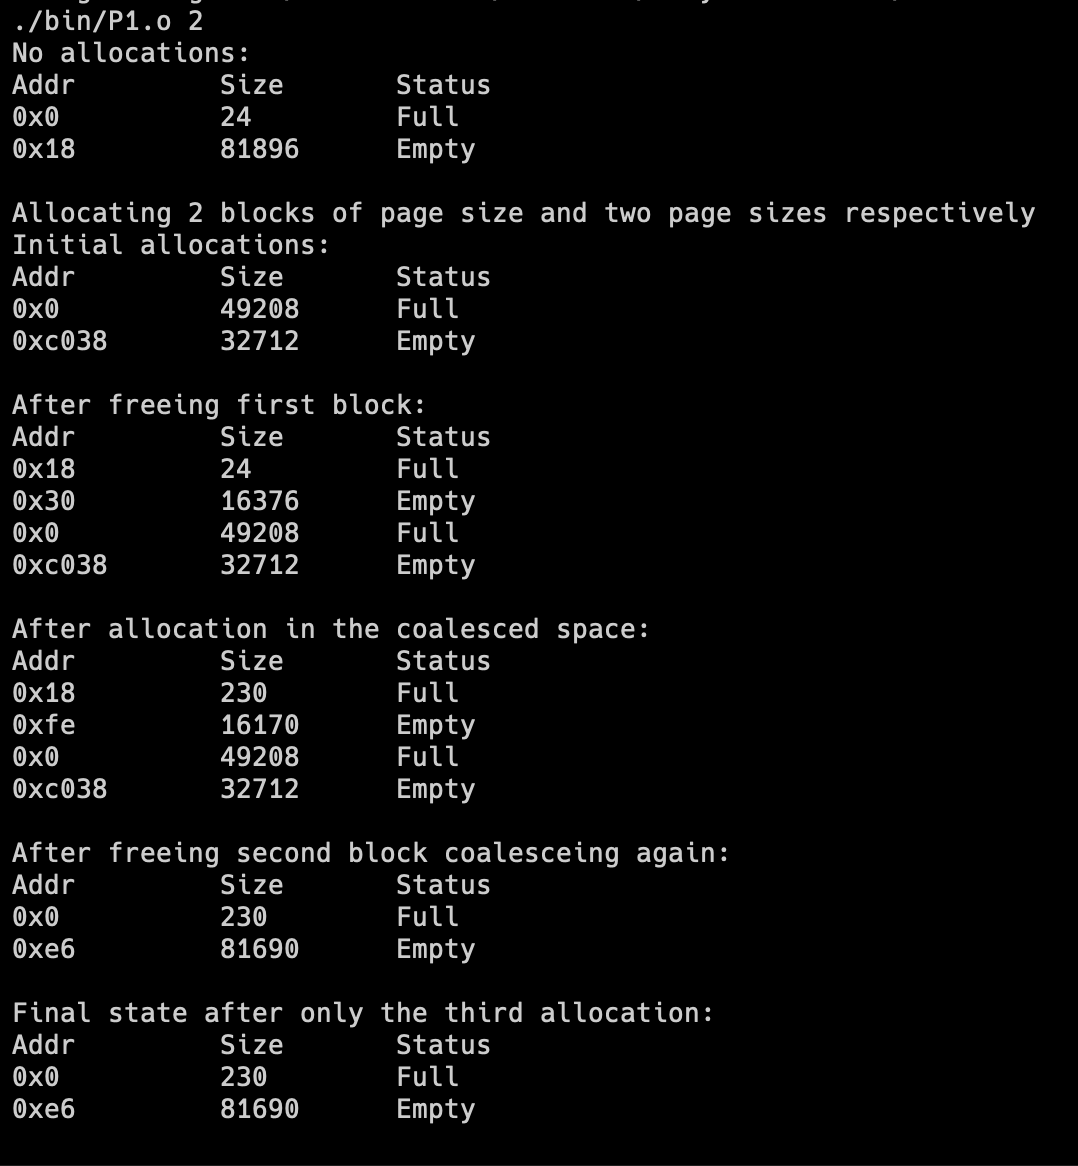
\includegraphics[width=\linewidth]{p1.png}
    \caption{Output for P1 using First Fit strategy}
\end{figure}
P1.c is very representative of the coalescing and reusing functions of MyMalloc as we can see both happening.
See Appendix for the full output of allprograms.c.

\section{Conclusion}
This report has detailed the development and testing of a custom memory management system designed to optimize allocation strategies like Bestfit, Worstfit, Firstfit, and Nextfit. While the system has demonstrated competence in managing dynamic memory allocation requests across various strategies, our analysis reveals that the coalescing mechanism requires further refinement to enhance its efficiency and effectiveness in real-world applications.

Additionally, the experimental unmap() function, currently in a beta stage, represents a promising enhancement to our memory management capabilities. Future work will focus on developing this function to fully integrate it into our system, aiming to improve the overall management of memory deallocation and system resource recovery.

Further research and development are necessary to address these areas, ensuring that our memory management system can meet the evolving needs of complex software environments more effectively.

\lstset{
    basicstyle=\ttfamily,
    breaklines=true,
    float=H,
    postbreak=\mbox{\textcolor{red}{$\hookrightarrow$}\space},
}

\appendix
Complete Program Output
\label{app:output}
\begin{lstlisting}[label={lst:firstLst},caption={Complete Program Output}]
./bin/allprograms.o
Enter the memory allocation strategy number (0-3): 0

Executing P1.o with strategy 0
No allocations:
Addr         Size       Status
0x0          24         Full
0x18         81896      Empty

Allocating 2 blocks of page size and two page sizes respectively
Initial allocations:
Addr         Size       Status
0x0          49208      Full
0xc038       32712      Empty

After freeing first block:
Addr         Size       Status
0x18         24         Full
0x30         16376      Empty
0x0          49208      Full
0xc038       32712      Empty

After allocation in the coalesced space:
Addr         Size       Status
0x18         230        Full
0xfe         16170      Empty
0x0          49208      Full
0xc038       32712      Empty

After freeing second block coalesceing again:
Addr         Size       Status
0x0          230        Full
0xe6         81690      Empty

Final state after only the third allocation:
Addr         Size       Status
0x0          230        Full
0xe6         81690      Empty

Program P1.o (PID: 25904) completed with exit status 0

Executing P2.o with strategy 0
No allocationsAddr         Size       Status
0x0          24         Full
0x18         16360      Empty

Allocating 4 blocks of size 3276 bytes using strategy 0
Addr         Size       Status
0x0          13192      Full
0x3388       3192       Empty

All allocations and deallocations successful.
Program P2.o (PID: 25905) completed with exit status 0

Executing P3.o with strategy 0
Addr         Size       Status
0x0          20584      Full
0x5068       28568      Empty

Addr         Size       Status
0x0          24         Full
0x18         49128      Empty

Addr         Size       Status
0x0          340        Full
0x154        48812      Empty

All allocations and deallocations successful.
Program P3.o (PID: 25906) completed with exit status 0

Executing P4.o with strategy 0
Initial allocations:
Addr         Size       Status
0x0          98392      Full
0x18058      81832      Empty

After freeing middle blocks:
Addr         Size       Status
0x4028       24         Full
0x4040       49160      Empty
0x0          98392      Full
0x18058      81832      Empty

After allocation in the coalesced space:
Addr         Size       Status
0x4028       24         Full
0x4040       49160      Empty
0x0          147560     Full
0x24068      32664      Empty

Final state after all deallocations:
Addr         Size       Status
0x0          24         Full
0x18         180200     Empty

Program P4.o (PID: 25907) completed with exit status 0
\end{lstlisting}


% trigger a \newpage just before the given reference
% number - used to balance the columns on the last page
% adjust value as needed - may need to be readjusted if
% the document is modified later
%\IEEEtriggeratref{8}
% The "triggered" command can be changed if desired:
%\IEEEtriggercmd{\enlargethispage{-5in}}

% references section

% can use a bibliography generated by BibTeX as a .bbl file
% BibTeX documentation can be easily obtained at:
% http://mirror.ctan.org/biblio/bibtex/contrib/doc/
% The IEEEtran BibTeX style support page is at:
% http://www.michaelshell.org/tex/ieeetran/bibtex/
%\bibliographystyle{IEEEtran}
% argument is your BibTeX string definitions and bibliography database(s)
%\bibliography{IEEEabrv,../bib/paper}
%
% <OR> manually copy in the resultant .bbl file
% set second argument of \begin to the number of references
% (used to reserve space for the reference number labels box)

% that's all folks
\end{document}


